%\documentclass[a4paper,twoside,10pt]{article}
\interfootnotelinepenalty=10000
\usepackage[USenglish]{babel} %francais, polish, spanish, ...
\usepackage[T1]{fontenc}
%\usepackage[ansinew]{inputenc}
\usepackage{color}
\usepackage{mathtools}
%\usepackage{hyperref}
\usepackage{subfig}
\usepackage{multirow, booktabs}
\usepackage{hyperref}


\usepackage{lmodern} %Type1-font for non-english texts and characters
\usepackage{algorithm}
\usepackage[noend]{algpseudocode}
\usepackage{mnsymbol}

%% Packages for Graphics & Figures %%%%%%%%%%%%%%%%%%%%%%%%%%
\usepackage{graphicx} %%For loading graphic files
\usepackage{amsmath}
\usepackage{amsthm} 
\usepackage{thmtools}
\usepackage{amsfonts}
\usepackage[all,cmtip]{xy}
\usepackage{tikz}

\usepackage{TechFront}
%\declaretheorem{Lemma}
%\declaretheorem{prop}

\newcommand{\lre}{\color{red}{\{}}

%\DeclareMathOperator{\sign}{sgn}
%\DeclareMathOperator{\coef}{coef}
%\DeclareMathOperator{\var}{var}
%\DeclareMathOperator{\eqs}{eqs}
%\DeclareMathOperator{\feas}{feas}
%\DeclareMathOperator{\UB}{UB}
%\DeclareMathOperator{\lb}{lb}
%\DeclareMathOperator{\FMcomb}{FM-comb}
%\DeclareMathOperator{\Gcomb}{Gauss-comb}
%\DeclareMathOperator{\proj}{proj}
%\DeclareMathOperator{\Pos}{Pos}
%\DeclareMathOperator{\Neg}{Neg}
%\DeclareMathOperator{\rhs}{rhs}
\newcommand{\sign}{\mathit{sgn}}
\newcommand{\coef}{\mathit{co}}
\newcommand{\var}{\mathit{var}}
\newcommand{\VAR}{\mathit{VAR}}
\newcommand{\eqs}{\mathit{eqs}}
\newcommand{\feas}{\mathit{feas}}
\newcommand{\UB}{\mathit{UB}}
\newcommand{\UBc}{\mathit{UBineq}}
\newcommand{\lb}{\mathit{lb}}
\newcommand{\lbc}{\mathit{lbineq}}
\newcommand{\FMcomb}{\mathit{FM}}
\newcommand{\Gcomb}{\mathit{GA}}
\newcommand{\proj}{\mathit{proj}}
\newcommand{\Pos}{\mathit{Pos}}
\newcommand{\Neg}{\mathit{Neg}}
\newcommand{\rhs}{\mathit{rhs}}
\newcommand{\bounds}{\mathit{bounds}}
\newcommand{\ie}{\mathcal{IE}}
\newcommand{\xx}{\mathcal{X}}
\newcommand{\vea}{\mathbf{co}}
\newcommand{\ttt}{\texttt{t}}
\newcommand{\trt}[1]{\texttt{#1}}
\newcommand{\mi}{\mathit}

\newcommand{\false}{\texttt{false}}
\newcommand{\true}{\texttt{true}}
\newcommand{\nul}{\texttt{null}}
\newcommand{\ve}{\mathbf}
%\newcommand\lhs[1]{\text{lhs}(#1)}
%\newcommand\rhs[1]{\text{rhs}(#1)}
%\newcommand\coef[1]{\text{coef}(#1)}
%\newcommand\LB[1]{\text{LB}_{#1}}
%\newcommand\UB[1]{\text{UB}_{#1}}
\newcommand{\lig}[4]{\ve{#1}\cdot\ve{#2}#3#4}
\newcommand\red[1]{\textcolor{red}{#1}}
\newcommand\blue[1]{\textcolor{blue}{#1}}
\newcommand{\set}[2]{\{\;{#1}\;|\;{#2}\;\}}
\newcommand{\odef}{\overset{\text{def.}}=}
\newcommand{\mc}{\mathcal}
\algdef{SE}[DOWHILE]{Do}{doWhile}{\algorithmicdo}[1]{\algorithmicwhile\ #1}%
\newcommand{\argmin}{\operatornamewithlimits{argmin}}
\newcommand{\StateInd}{\State\hspace{\algorithmicindent}}
\newcommand{\pr}{\mathit{PR}}
\newcommand{\prs}{\mathit{PRS}}
\newcommand{\ens}{\Leftrightarrow}

%\algdef{SE}[DOPAR]{DoPar}{doParWhile}{\algorithmicdo\textbf{ in parallel for\ }}[1]{\algorithmicwhile\ #1}%
\algdef{SE}[DOPAR]{DoPar}{doParUntil}{\algorithmicdo\textbf{ in parallel for\ }}[1]{\algorithmicuntil\ #1}%

\algdef{SE}[SUBALG]{Indent}{EndIndent}{}{\algorithmicend\ }%
\algtext*{Indent}
\algtext*{EndIndent}

\newtheorem{prop}{Proposition}
\newtheorem{lemma}{Lemma}
\newtheorem{cor}{Corollary}

\newcounter{para}
%\newcommand\mypara[1]{\par\refstepcounter{para}\textbf{\thep‌​ara\space#1\space}}
\newcommand\mypara[1]{\newline\par\refstepcounter{para}\textbf{\thepara}\space \textbf{#1} \space}
%\newcommand\mypara{\par\refstepcounter{para}\thepara\space}
%\usepackage[thmmarks,...]{ntheorem}
\newcommand{\Sec}{F}
\newcommand{\Ca}{\mi{Cap}}
\newcommand{\Vol}{\mi{V}}
\newcommand{\Weight}{\mi{W}}
\newcommand{\weight}{\mi{w}}
\newcommand{\BonjeanStations}{\mi{BS}}
\newcommand{\bonjean}{bf}
\newcommand{\Bonj}{B}
\newcommand{\shear}{\mi{sf}}
\newcommand{\Prop}{P}

\theoremstyle{definition}
%\newtheorem{example}{Example}[section]
\newtheorem*{theorem}{Theorem}

\theoremstyle{definition}
\newtheorem{examplex}{Example}[section]
\newenvironment{example}
  {\pushQED{\qed}\renewcommand{\qedsymbol}{$\triangle$}\examplex}
  {\popQED\endexamplex}
	
%\newtheoremstyle{named}{}{}{\itshape}{}{\bfseries}{.}{.5em}{\thmnote{#3}}
%\theoremstyle{named}
%\newtheorem*{namedtheorem}{Theorem}

%\begin{document}
\section{Definitions and notation}
%\paragraph{Constraint systems}
In the following, a constraint system $S$ is a set of equalities and inequalities over the same set of variables, $\VAR(S)=\{x_1,\ldots, x_n\}$. 
Each constraint $c$ is either an equality, written $a_1x_1 + \ldots +a_nx_n = b$, or an inequality, written $a'_1x_1 + \ldots +a'_nx_n\leq b'$. Though, the left-hand-side is also written using a dot-product. 
%
We let $\var(c)$ denote the variables whose coefficient in $c$ is nonzero and say that $c$ \emph{uses} $x$ if $x\in \var(c)$.

The set of points in $\mathbb{R}^{|\VAR(S)|}$ that satisfies all constraints in $S$ is called $S$'s \emph{feasible area}. A constraint $c\in S$ is \emph{redundant} if it does not influence the feasible area for $S$. In other words the inequality $c: \ve{a}\cdot\ve{x}\leq b$ is redundant iff $\max \ve{a}\cdot\ve{x}$ w.r.t. $S\setminus\{c\}$ is less or equal to $b$.
An equality is redundant iff both corresponding inequalities are redundant.
If the constraint $c$ is \emph{not} redundant, it is called \emph{non-redundant} or binding.

%\paragraph{Projection}
As described, the feasible area of $S$ describes the combination of values for the variables in $\VAR(S)$ that satisfy all constraints in $S$. However, there are some variables $Y\subseteq \VAR(S)$ whose value in a feasible point we are not interested in; we just want to know that a satisfying value exists. This information is captured by the \emph{projection} of the feasible area of $S$ w.r.t. $Y$, $\mi{proj}_YS\in\mathbb{R}^{|\VAR(S)\setminus Y|}$. This is the largest set consisting of values for $\VAR(S)\setminus Y$ that can be extended with values for $Y$ such that all constraints in $S$ are satisfied (see Figure~\ref{fig:proj}). 

\begin{figure}
	\centering
		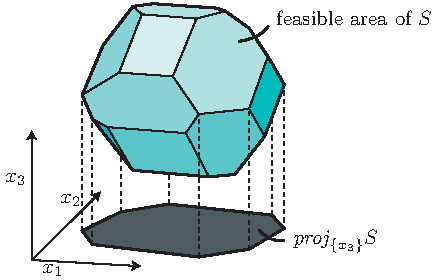
\includegraphics[scale=0.8]{figures/projection2.pdf}
	\caption{The projection of the system $S$ with respect to $\{x_3\}$.}
	\label{fig:proj}
\end{figure}

The projection of a system $S$ is a set of points in Euclidian space, and it is the feasible region of (another) system $S'$ (see e.g. \cite{ziegler95}). However, many constraint systems determine the same feasible area, and when we say e.g. ``$S'$ is the projection of $S$ w.r.t. $Y$'' we mean that ``$S'$ is one of the constraint systems whose feasible area equals the projection of the feasible area of $S$ w.r.t $Y$''.

%\paragraph{A note on $\VAR(S)$}
In this paper, we are mainly interested in the original system $S$ and its projection $S'$, while the associated feasible areas of $S$ and $S'$ are the ``mediator'' between the two systems. 
However, since the feasible area of a system is just a set of points in a multi-dimensional Euclidian space, the number and the order of the variables are important and needs to be given (explicitly or implicitly). 
%
Though, the inequality $c:a_1x_1\leq b$ can be considered both as an inequality over the set $\{x_1\}$ as well as over any set $X$ where $x_1\in X$, and we will not specify $VAR(S')$ formally for every considered constraint system $S$.
Intuitively, we just make sure that the dimensions (and order of variables) ``match''. For example, when two systems $T$ and $T'$ are joined to form another system $T''$, we consider $T$ and $T'$ as constraints over the same variable set, $VAR(T'')=var(T)\cup var(T')$.
A more stringent exposition keeping track of the variable sets and ordering can be found in \cite{MyTechRep}.
%\end{document}
